\section{Улучшение качества компилированной речи}

\subsection{Задание 3.3.4. Правка осциллограммы}

Для улучшения выбрана фраза <<Ты дома.>>. Сравнение осциллограмм эталона и
фонемной компиляции показало две основные причины искажений:
\begin{itemize}
	\item неудачные экземпляры гласных [ы] (205~Гц) и [о] (145~Гц),
	произнесённые с восходящей интонацией списка; они заменены ядрами тех
	же фонем, вырезанными из слогов <<ты>> (143~Гц) и <<до>> (125~Гц),
	где тон устойчив;
	\item резкие стыки между сегментами; они сглажены перекрёстным
	затуханием 10~мс, в начале и конце фразы добавлены плавные фронты
	(8 и 40~мс).
\end{itemize}
Дополнительно уточнены длительности и уровни всех сегментов. Результаты
приведены в таблице~\ref{tab:improved} и на
рисунках~\ref{fig:improved-wave},~\ref{fig:improved-f0}.

\begin{table}[H]
	\centering
	\small
	\caption{Улучшение фразы <<Ты дома.>> (задание 3.3.4)}
	\label{tab:improved}
	\begin{tabular}{|l|c|c|c|c|}
		\hline
		Вариант & Длит., с & Пик / RMS, дБFS &
		$F_0$ мед., Гц & Скачок $F_0$, Гц \\
		\hline
		эталон & 0,52 & $-9{,}0$ / $-22{,}6$ & 132 & 6 \\
		\hline
		компиляция из фонем & 0,71 & $-6{,}0$ / $-16{,}0$ & 126 & 35 \\
		\hline
		после правки & 0,71 & $-6{,}0$ / $-17{,}4$ & 130 & 15 \\
		\hline
	\end{tabular}
\end{table}

\begin{figure}[H]
	\centering
	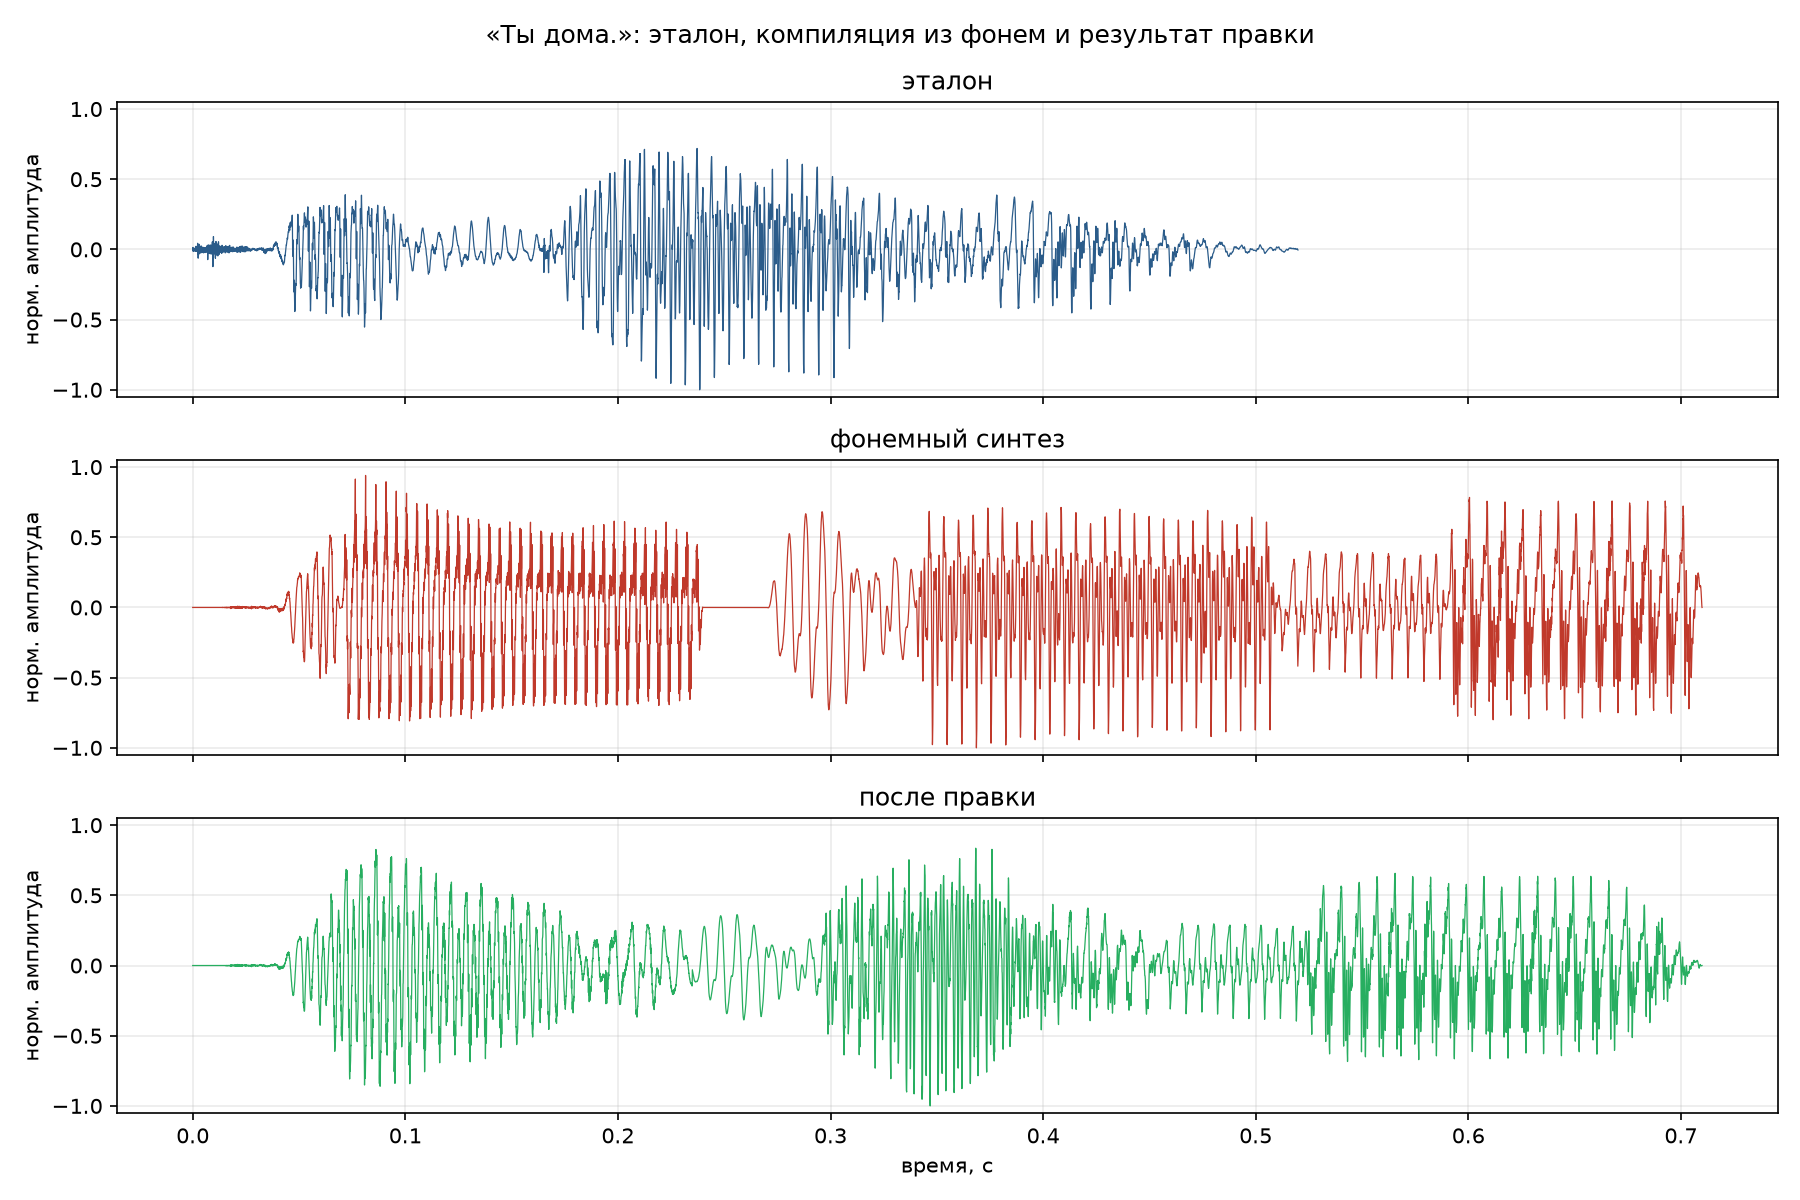
\includegraphics[width=\textwidth]{lab3_improved_wave.png}
	\caption{Осциллограммы фразы <<Ты дома.>>: эталон, компиляция из фонем
		и результат правки}
	\label{fig:improved-wave}
\end{figure}

\begin{figure}[H]
	\centering
	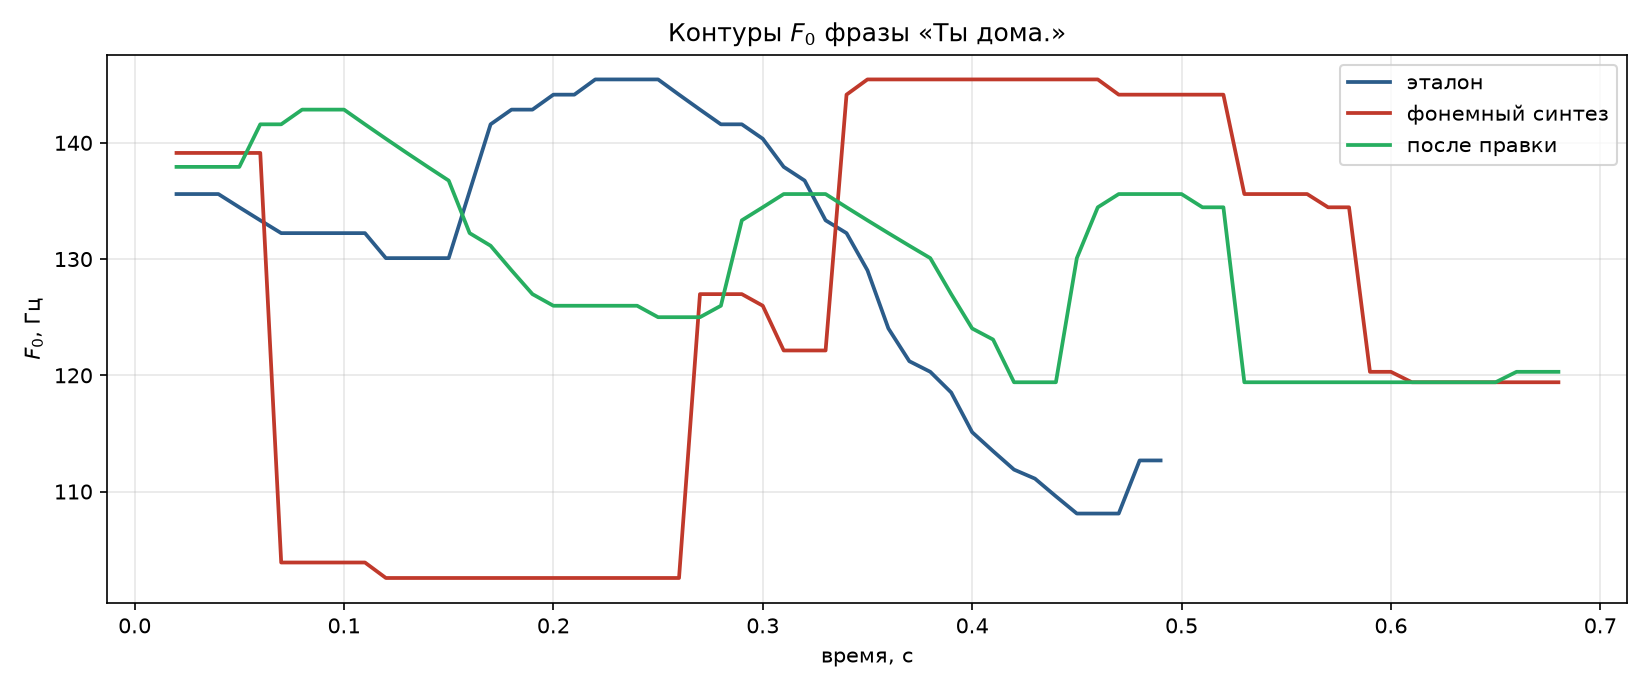
\includegraphics[width=\textwidth]{lab3_improved_f0.png}
	\caption{Контуры $F_0$ фразы <<Ты дома.>> до и после правки}
	\label{fig:improved-f0}
\end{figure}

После правки максимальный скачок $F_0$ уменьшился с 35 до 15~Гц, диапазон
изменения тона сузился (119--143~Гц вместо 103--145~Гц), а медиана
приблизилась к эталонной (130 против 132~Гц). Фраза стала звучать заметно
естественнее, хотя по-прежнему остаётся монотонной по сравнению с
эталоном, имеющим нисходящий мелодический контур.

\subsection{Задание 3.3.5. Компиляция фраз из слогов}

Дальнейшее улучшение достигнуто совершенствованием фонетической базы:
вместо отдельных фонем записаны и использованы целые слоги
<<ма мы ла ра му па и я ты до>> (файлы \texttt{syl\_01.wav}--\texttt{syl\_10.wav},
рис.~\ref{fig:syllables}). Слог сохраняет естественный переход
<<согласный--гласный>> (коартикуляцию), поэтому стыки внутри слога не
разрушаются при компиляции. Характеристики слогов приведены в
таблице~\ref{tab:syllables}, результаты компиляции фраз --- в
таблице~\ref{tab:sylres}.

\begin{table}[H]
	\centering
	\footnotesize
	\caption{Характеристики слогов (задание 3.3.5)}
	\label{tab:syllables}
	\begin{tabular}{|l|c|c|c|c|c|c|c|c|c|c|}
		\hline
		Слог & ма & мы & ла & ра & му & па & и & я & ты & до \\
		\hline
		Длит., с & 0,30 & 0,28 & 0,30 & 0,28 & 0,30 & 0,25 & 0,18 & 0,30 & 0,26 & 0,30 \\
		\hline
		RMS & $-18{,}0$ & $-18{,}0$ & $-20{,}0$ & $-18{,}0$ & $-20{,}0$ & $-20{,}0$ & $-20{,}0$ & $-18{,}0$ & $-20{,}0$ & $-18{,}0$ \\
		\hline
		$F_0$, Гц & 135 & 138 & 133 & 132 & 140 & 134 & 134 & 130 & 140 & 127 \\
		\hline
	\end{tabular}
\end{table}

\begin{figure}[H]
	\centering
	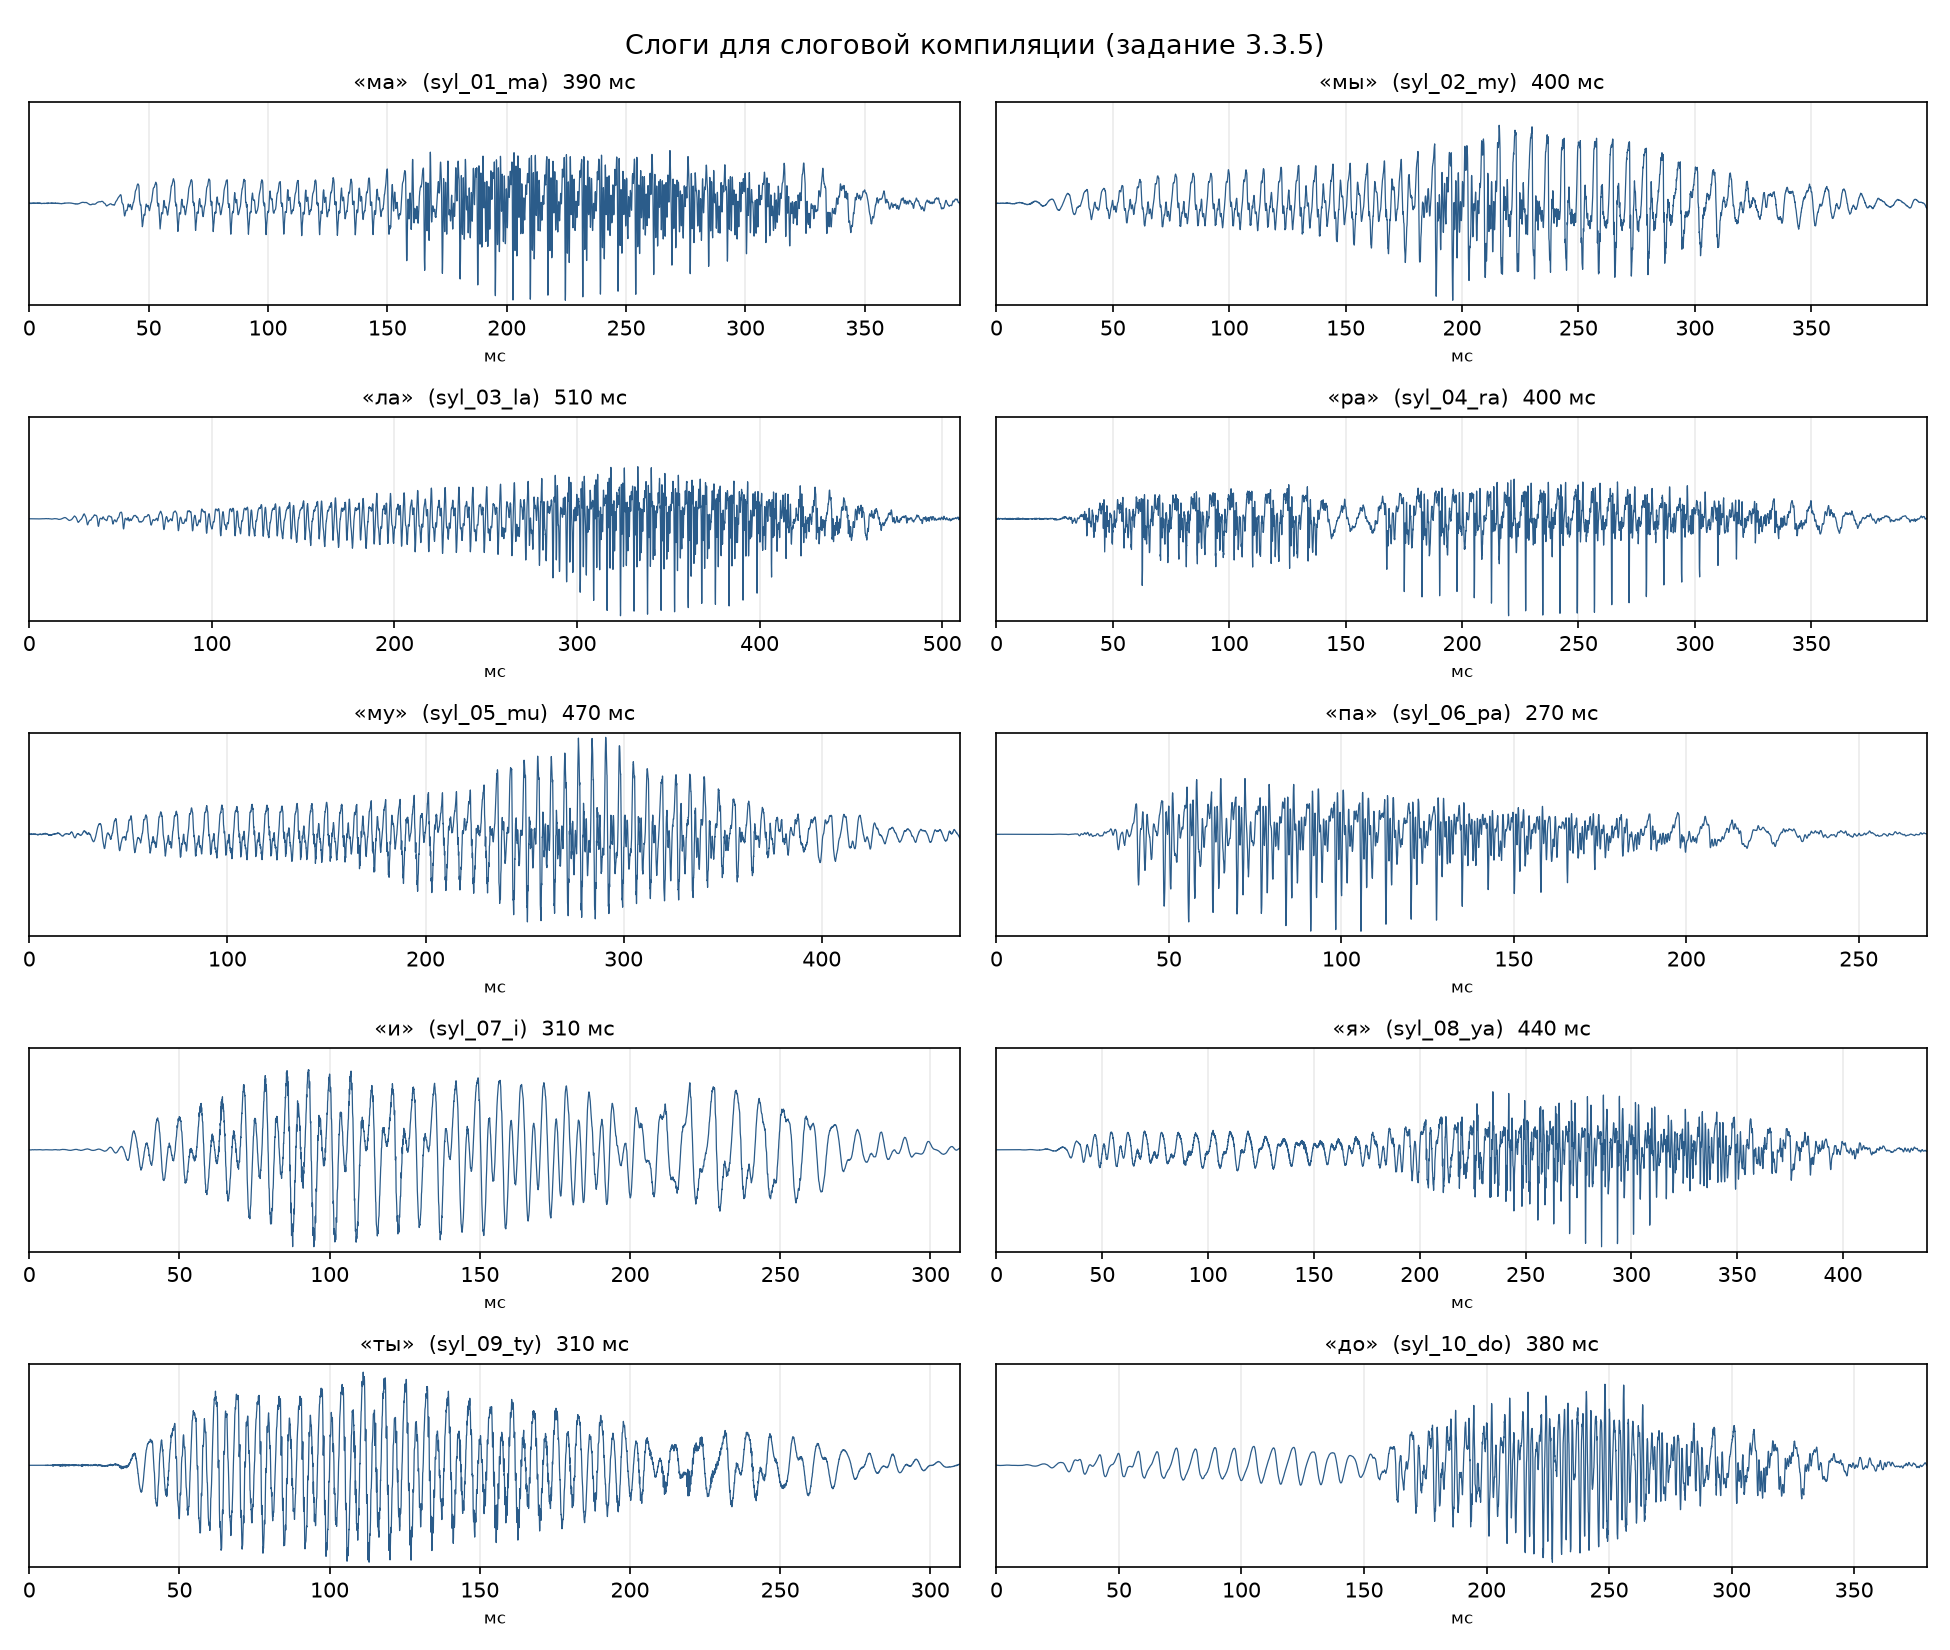
\includegraphics[width=\textwidth]{lab3_syllables.png}
	\caption{Осциллограммы слогов для слоговой компиляции}
	\label{fig:syllables}
\end{figure}

\begin{table}[H]
	\centering
	\small
	\caption{Фразы, скомпилированные из слогов}
	\label{tab:sylres}
	\begin{tabular}{|l|c|c|c|}
		\hline
		Фраза & Длит., с & $F_0$ мед., Гц & Скачок $F_0$, Гц \\
		\hline
		<<Мама мыла раму.>> & 1,90 & 134 & 6 \\
		\hline
		<<Мама, папа и я.>> & 2,31 & 132 & 13 \\
		\hline
		<<Ты дома?>> & 0,87 & 133 & 11 \\
		\hline
		<<Ты дома.>> & 0,87 & 133 & 11 \\
		\hline
	\end{tabular}
\end{table}

Сравнение с фонемной компиляцией (таблица~\ref{tab:compare}) показывает
преимущества слоговой базы:
\begin{itemize}
	\item максимальный скачок $F_0$ уменьшился в 3--8 раз (с 35--100 до
	6--13~Гц), так как тон внутри слога стабилен и переходы естественны;
	\item диапазон изменения $F_0$ приблизился к эталонному
	(например, для фразы~1 --- 121--145~Гц против 103--172~Гц у фонемной
	компиляции);
	\item средний уровень стал ближе к эталону ($-20\dots-23$~дБFS против
	$-16$~дБFS), поскольку слог целиком нормировался к типовому уровню.
\end{itemize}
Однако обе компиляции по-прежнему монотонны: вопрос и утверждение,
составленные из одинаковых слогов, звучат одинаково. Это показывает, что
при разработке синтезаторов необходимо учитывать не только фонетические,
но и просодические особенности речи --- мелодику, ритмику и энергетику,
которым посвящено следующее задание.

\begin{figure}[H]
	\centering
	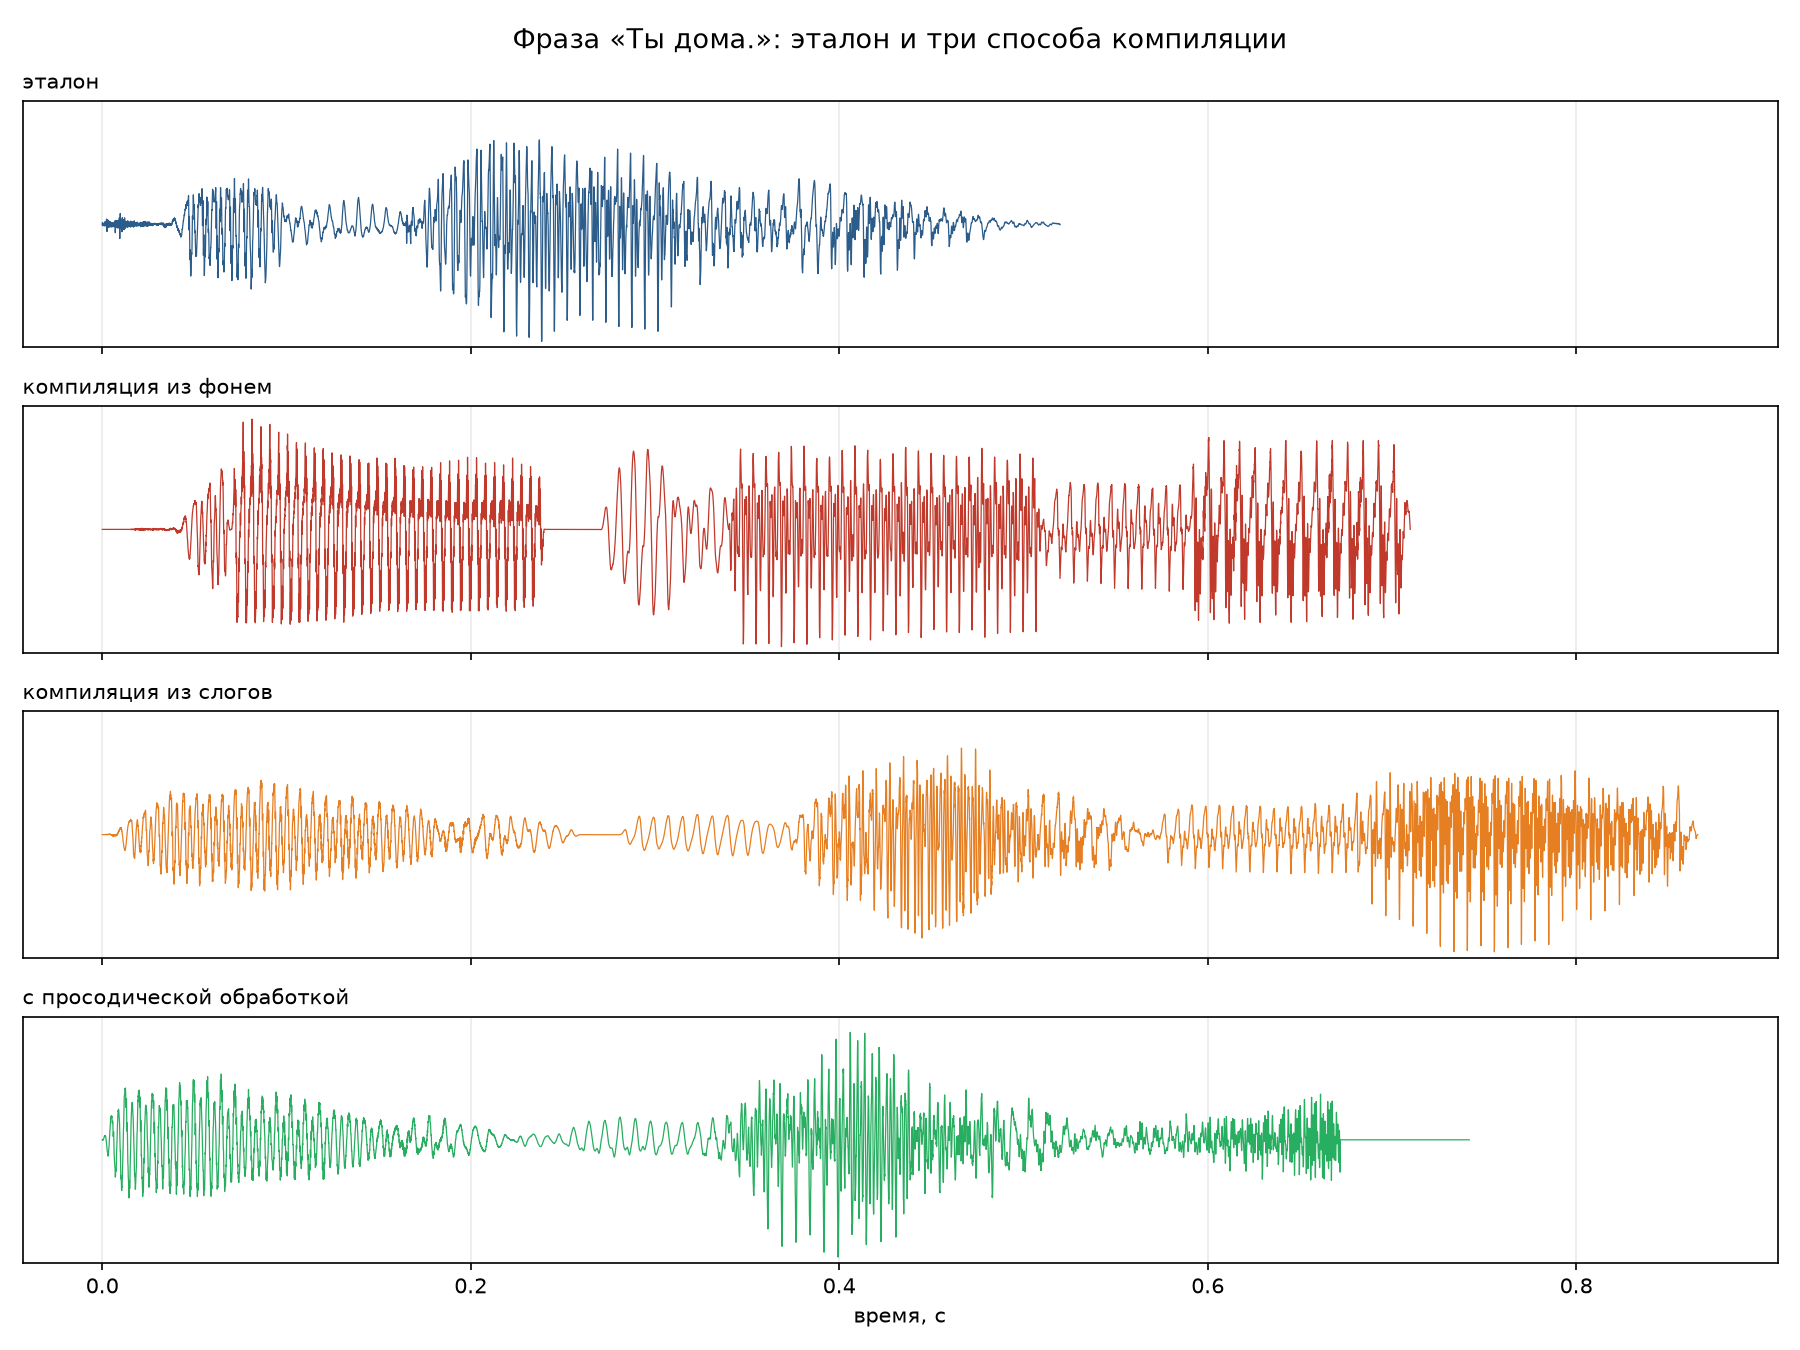
\includegraphics[width=\textwidth]{lab3_variants_compare.png}
	\caption{Фраза <<Ты дома.>>: эталон и три способа компиляции}
	\label{fig:variants}
\end{figure}
